\documentclass[a4paper,11pt]{report}

\usepackage{fullpage}

\usepackage{amsmath}
\usepackage{bussproofs}
\usepackage{mathpartir}
\usepackage{prooftrees}
\usepackage{color}
\usepackage{hyperref}
\usepackage{placeins}


% for finite state automata
\usepackage{tikz}
\usetikzlibrary{automata,positioning}

%%%%%%%%%%%%%%%%%%%%%%%%%%%%%%%%%%%%%%%%%%%%%%%%%%%%%%%%%
% Minted
%%%%%%%%%%%%%%%%%%%%%%%%%%%%%%%%%%%%%%%%%%%%%%%%%%%%%%%%%

\usepackage[cache=false]{minted}

%%%%%%%%%% C
\newmintinline{c}{
  fontsize=\small,
  breaklines=true
}

\newminted{c}{
  frame=single,
  framesep=2mm,
  fontsize=\scriptsize,
  mathescape
}

\newminted[ccodeline]{c}{
  frame=single,
  framesep=2mm,
  fontsize=\scriptsize,
  mathescape,
  linenos
}


%%%%%%%%% CMAKE
\newminted{cmake}{
  frame=single,
  framesep=2mm,
  fontsize=\scriptsize,
  mathescape,
  linenos,
  breaklines=true
}

% End minted
%%%%%%%%%%%%%%%%%%%%%%%%%%%%%%%%%%%%%%%%%%%%%%%%%%%%%%%%%


\author{Sylvain Julmy}
\date{\today}

\setlength{\parindent}{0pt}

\begin{document}

\begin{center}
  \Large{
    Operating Systems\\
    Spring 2018
  }
  
  \noindent\makebox[\linewidth]{\rule{\linewidth}{0.4pt}}
  S04
  \noindent\makebox[\linewidth]{\rule{\linewidth}{0.4pt}}

  \begin{flushleft}
    Professor : Philippe Cudré-Mauroux

    Assistant : Ines Arous
  \end{flushleft}
  
  \noindent\makebox[\linewidth]{\rule{\linewidth}{0.4pt}}

  Submitted by Sylvain Julmy
  
  \noindent\makebox[\linewidth]{\rule{\textwidth}{1pt}}
\end{center}

\section*{Exercice 2}

\begin{figure}[ht]
  \centering
  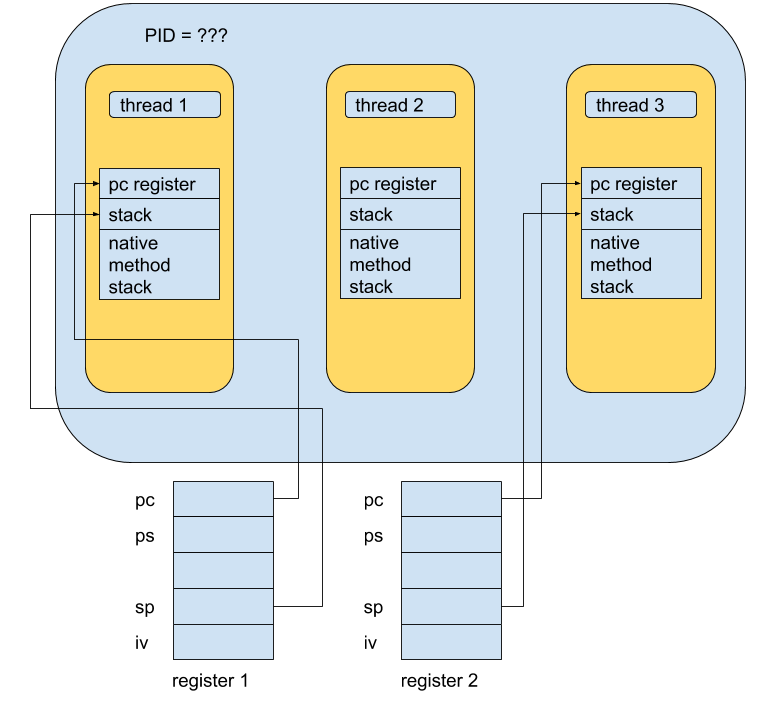
\includegraphics[width=0.5\textwidth]{figures/OS_s04_ex2}
  \caption{\label{fig:label}Thread memory model.}
\end{figure}

\FloatBarrier

\section*{Exercice 3}

Is it possible to force each thread to wait on a certain message before
continuing their execution. We can synchronize the thread using, for example,
\verb+pthread_cond_wait()+.

If it is not possible to synchronize the thread, we can always hack the kernel
scheduler and add our own algorithm...

\section*{Exercice 4}

The source code for both version is available in appendix.

\end{document}
